\subsection{Sequence Diagram}

\begin{figure}[h]
    \centering
    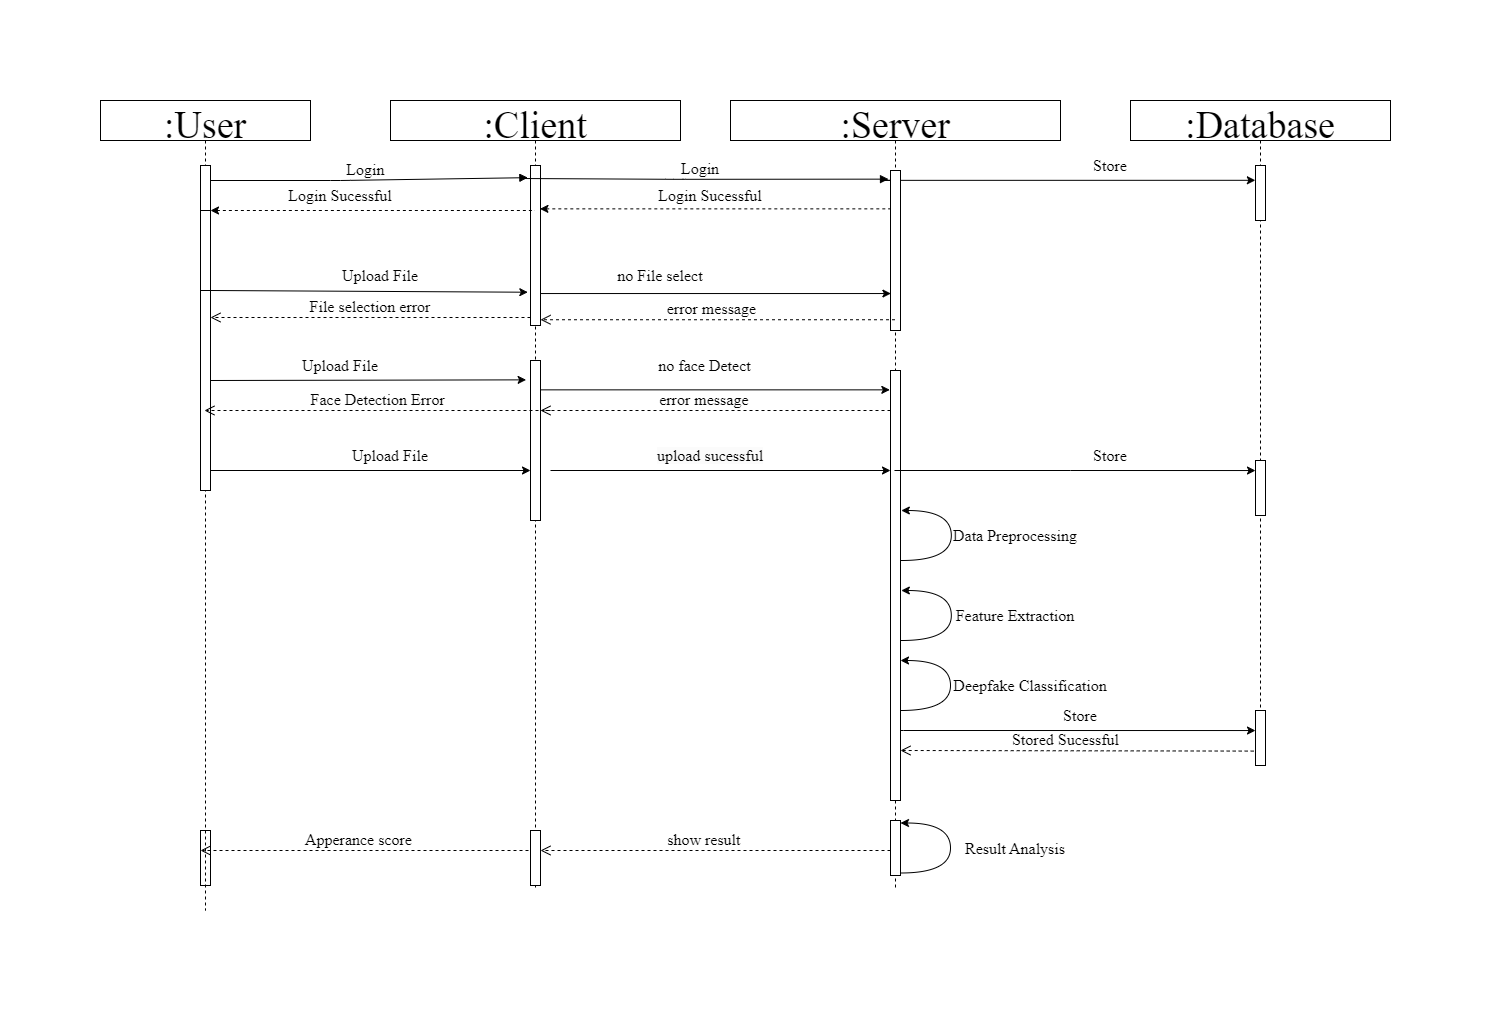
\includegraphics[width=8in]{img/sequencediagram.drawio.png}
    \caption{\textit{Sequence Diagram}}
\end{figure}

\justify
The sequence diagram shows that the user initiates the process by accessing the system and providing their login credentials. The Server checks the login credentials and verifies the user's identity. Once authenticated, the user proceeds to upload a file containing the video or image to be analyzed for deepfakes. Then face detection algorithms are used to detect and extract faces from the uploaded media. This collected data undergoes further processing, including resizing and normalization, to prepare it for deep learning modeling. Finally, the processed data is fed into the deep learning model, which analyzes the features and patterns to classify the media as either real or fake.
